\documentclass[bimj,fleqn]{w-art}
\usepackage{times}
\usepackage{w-thm}
\usepackage[authoryear]{natbib}
\setlength{\bibsep}{2pt}
\setlength{\bibhang}{2em}
\newcommand{\J}{J\"{o}reskog}
\newcommand{\So}{S\"{o}rbom}
\newcommand{\bcx}{{\bf X}}
\newcommand{\bcy}{{\bf Y}}
\newcommand{\bcz}{{\bf Z}}
\newcommand{\bcu}{{\bf U}}
\newcommand{\bcv}{{\bf V}}
\newcommand{\bcw}{{\bf W}}
\newcommand{\bci}{{\bf I}}
\newcommand{\bch}{{\bf H}}
\newcommand{\bcb}{{\bf B}}
\newcommand{\bcr}{{\bf R}}
\newcommand{\bcm}{{\bf M}}
\newcommand{\bcf}{{\bf F}}
\newcommand{\bcg}{{\bf G}}
\newcommand{\bcs}{{\bf S}}
\newcommand{\bca}{{\bf A}}
\newcommand{\bcd}{{\bf D}}
\newcommand{\bcc}{{\bf C}}
\newcommand{\bce}{{\bf E}}
\newcommand{\ba}{{\bf a}}
\newcommand{\bb}{{\bf b}}
\newcommand{\bc}{{\bf c}}
\newcommand{\bd}{{\bf d}}
\newcommand{\bx}{{\bf x}}
\newcommand{\by}{{\bf y}}
\newcommand{\bz}{{\bf z}}
\newcommand{\bu}{{\bf u}}
\newcommand{\bv}{{\bf v}}
\newcommand{\bh}{{\bf h}}
\newcommand{\bl}{{\bf l}}
\newcommand{\be}{{\bf e}}
\newcommand{\br}{{\bf r}}
\newcommand{\bw}{{\bf w}}
\newcommand{\de}{\stackrel{D}{=}}
\newcommand{\bt}{\bigtriangleup}
\newcommand{\bfequiv}{\mbox{\boldmath $\equiv$}}
\newcommand{\bmu}{\mbox{\boldmath $\mu$}}
\newcommand{\bnu}{\mbox{\boldmath $\nu$}}
\newcommand{\bxi}{\mbox{\boldmath $\xi$}}
\newcommand{\btau}{\mbox{\boldmath $\tau$}}
\newcommand{\bgamma}{\mbox{\boldmath $\Gamma$}}
\newcommand{\bphi}{\mbox{\boldmath $\Phi$}}
\newcommand{\bfphi}{\mbox{\boldmath $\varphi$}}
\newcommand{\bfeta}{\mbox{\boldmath $\eta$}}
\newcommand{\bpi}{\mbox{\boldmath $\Pi$}}
\newcommand{\bequiv}{\mbox{\boldmath $\equiv$}}
\newcommand{\bvarepsilon}{\mbox{\boldmath $\varepsilon$}}
\newcommand{\btriangle}{\mbox{\boldmath $\triangle$}}
\newcommand{\bdelta}{\mbox{\boldmath $\Delta$}}
\newcommand{\beps}{\mbox{\boldmath $\epsilon$}}
\newcommand{\btheta}{\mbox{\boldmath $\theta$}}
\newcommand{\balpha}{\mbox{\boldmath $\alpha$}}
\newcommand{\bsphi}{\mbox{\boldmath $\varphi$}}
\newcommand{\bsig}{\mbox{\boldmath $\sigma$}}
\newcommand{\bfpsi}{\mbox{\boldmath $\psi$}}
\newcommand{\bfdelta}{\mbox{\boldmath $\delta$}}
\newcommand{\bsigma}{{\bf \Sigma}}
\newcommand{\bzero}{{\bf 0}}
\newcommand{\bpsi}{\mbox{\boldmath $\Psi$}}
\newcommand{\bep}{\mbox{\boldmath $\epsilon$}}
\newcommand{\bomega}{\mbox{\boldmath $\Omega$}}
\newcommand{\bfomega}{\mbox{\boldmath $\omega$}}
\newcommand{\blambda}{\mbox{\boldmath $\Lambda$}}
\newcommand{\bflambda}{\mbox{\boldmath $\lambda$}}
\newcommand{\bfsigma}{\mbox{\boldmath $\sigma$}}
\newcommand{\bfpi}{{\mbox{\boldmath $\pi$}}}
\newcommand{\bupsilon}{\mbox{\boldmath $\upsilon$}}
\newcommand{\obs}{{\rm obs}}
\newcommand{\mis}{{\rm mis}}
\theoremstyle{plain}
\newtheorem{criterion}{Criterion}
\theoremstyle{definition}
\newtheorem{condition}[theorem]{Condition}
\usepackage[]{graphicx}
\chardef\bslash=`\\ % p. 424, TeXbook
\newcommand{\ntt}{\normalfont\ttfamily}
\newcommand{\cn}[1]{{\protect\ntt\bslash#1}}
\newcommand{\pkg}[1]{{\protect\ntt#1}}
\let\fn\pkg
\let\env\pkg
\let\opt\pkg
\hfuzz1pc % Don't bother to report overfull boxes if overage is < 1pc
\newcommand{\envert}[1]{\left\lvert#1\right\rvert}
\let\abs=\envert

\begin{document}
%\DOIsuffix{bimj.DOIsuffix}
\DOIsuffix{bimj.200100000}
\Volume{52}
\Issue{61}
\Year{2010}
\pagespan{1}{}
\keywords{Evaluation; Imputation; Missing data; Simulation studies;\\[1pc]
\noindent \hspace*{-4.2pc} Supporting Information for this article is available from Github, \break \hspace*{-4pc} \underline{github.com/gerkovink/StandardizedEvaluation}.
}  %%% semicolon and fullpoint added here for keyword style

\title[Standardized evaluation]{Towards a standardized evaluation of imputation methodology}
%% Information for the first author.
\author[Oberman]{Hanne I. Oberman\footnote{Corresponding author: {\sf{e-mail: h.i.oberman@uu.nl}}}\inst{,1}} 
\address[\inst{1}]{Departement of Methodology \& Statistics, Padualaan 14, 3584 CH Utrecht, The Netherlands}
%%%%    Information for the second author
\author[Vink]{Gerko Vink\inst{1}}
%%%%    \dedicatory{This is a dedicatory.}
\Receiveddate{zzz} \Reviseddate{zzz} \Accepteddate{zzz} 

\begin{abstract}
Developing new imputation methodology has become a very active field. Unfortunately, there is no consensus on how to perform simulation studies to evaluate the properties of imputation methods. In this paper we propose a move towards a standardized evaluation of imputation methods. To demonstrate the need for standardization, we highlight a set of potential pitfalls that bring forth a chain of potential problems in the objective assessment of the performance of imputation routines. This may lead to suboptimal use of multiple imputation in practice. Additionally, we suggest a course of action for simulating and evaluating missing data problems.
\end{abstract}



%% maketitle must follow the abstract.
\maketitle                   % Produces the title.

%% If there is not enough space inside the running head
%% for all authors including the title you may provide
%% the leftmark in one of the following three forms:

%% \renewcommand{\leftmark}
%% {First Author: A Short Title}

%% \renewcommand{\leftmark}
%% {First Author and Second Author: A Short Title}

%% \renewcommand{\leftmark}
%% {First Author et al.: A Short Title}

%% \tableofcontents  % Produces the table of contents.

%%%%%%%%%%%%%%%%%%%%%%%%%%
%% INTRODUCTION
%%%%%%%%%%%%%%%%%%%%%%%%%%

\section{Introduction}

Imputation is a state-of-the-art technique for drawing valid conclusions from incomplete data. The technique has earned a permanent spot in research and policy making, demonstrated e.g. by the detailed manual created by the National Research Council \citep*{little2012prevention}. Although a top-down enforcement of valid ways to handle missing data is not yet very pronounced, an increasing amount of researchers are embracing imputation techniques. After all, the principle of imputation is very intuitive.

The idea behind imputation is to impute (fill in) missing data, to obtain a valid estimate of what could have been. A popular variant is multiple imputation \citep{rubi76}, whereby each missing value is imputed multiple times. The completed data that are thus obtained can be analyzed by standard techniques and, in the case of multiple imputation, the analysis results can be combined into a single inference \citep[using Rubin's rules][]{rubi87}. In contrast to ad hoc methods for dealing with missing values (e.g. list-wise deletion, mean imputation, regression imputation, last observation carried forward, indicator method), multiple imputation properly takes into account the sources of uncertainty that are related to the missingness problem. 

The quality of a solution obtained by imputation depends on the statistical properties of the incomplete data and the degree to which an imputation procedure is able to capture these properties when modeling missing values. In general it holds that modeling missing data becomes more challenging when the amount of missingness increases [ref?]. However, when (strong) relations in the data are present, the observed parts can hold great predictive power for the models that estimate the missingness. In that case,  imputation would be substantially more efficient than the ubiquitous list-wise deletion.

When evaluating the statistical properties (and thereby the practical applicability) of imputation methodology, researchers most often make use of simulation studies. In such studies a complete dataset is usually generated from a statistical model, another model is used to induce missingness, and a set of evaluation criteria is postulated to evaluate the performance of one or more missing data methods. However, no golden standard has been established to evaluate imputation routines and, as a result, the validity of the simulation procedures may differ tremendously from one developer to another. Especially with novel imputation methods being propagated from the fields of machine learning and artificial intelligence, the differences may become more pronounced. Although these promising new methods seem to yield even sharper imputations than now-standard (semi-)parametric imputation methods, the comparison may not be fair due to the simulation setup. 

% [Nowadays there are a lot of imp alg being propagated, esp ai/ml, whose perf often times seems quite promising. But may not be a fair comparison because of the simulation set-up/dev in ai/ml so fast that steps may be skipped. Especially in the field of ML/AI, there are promising new imputation methods, which may yield even sharper imputations than now-standard (semi-)parametric imputation methods]

The purpose of this paper is threefold: First, to raise some concerns with respect to evaluating imputation methodology. These concerns stem from careful consideration with fellow 'imputers' and from encounters as a reviewer for statistical journals. Second, to provide imputation methodologists with a suggested course of action when simulating missing data problems. This suggested approach should identify a common ground, but is in no way intended as an absolute solution. This identifies the third purpose of this paper: discussion. We hope to elicit critical thinking with respect to the problems at hand. We are all convinced that our methodology has some merit. But for sake of progress it would be much more advantageous if the aim of our evaluations would go beyond \emph{proving the point} and would legitimately consider the statistical properties. 


%%%%%%%%%%%%%%%%%%%%%%%%%%
%% PROBLEMS
%%%%%%%%%%%%%%%%%%%%%%%%%%

\section{Why some evaluations should not be trusted}

As of today, there is no consensus on how to perform simulation studies to evaluate the properties of imputation methods. Typically, the developer of a new imputation routine does some tests by simulations, but these tests differ across developers. This brings forth a chain of potential problems in the objective assessment of imputation method performance, within and across studies, which may lead to sub-optimal use of imputation in practice. To demonstrate the broad impact of these problems, we subdivide the problems in the following three distinct categories: problems with data generation, problems with missingness generation and problems with performance evaluation. We further detail the impact these problems may have on the validity of the performance evaluation of the imputation routines [this sentance could be smoother]. 

%%%%%%%%%%%%%%%%%%%%%%%%%%

\subsection{Data generation problems}

To evaluate the ability of an imputation routine to handle missingness, a form of truth has to be established. Those who perform simulation studies are in the luxury position to establish the truth beforehand by choosing a data generating mechanism. Data generating mechanisms define how a complete dataset is obtained at the start of each simulation repetition. There are two general approaches to generaring complete data: (i) model-based simulation, in which data are drawn from a known statistical model or probability distribution, such as the multivariate normal distribution; and (ii) design-based simulation, where data are sampled (with replacement) from a sufficiently large observed set, such as from official statistics records.

The problem with model-based data generating mechanisms is that a method's performance on simulated data may not translate to empirical data. Real-life data hardly ever follow a given theoretical distribution, so there is no guarantee that simulation results are generalizable. Moreover, data are often generated such that the problem that is being studied is most pronounced, e.g. with consistently high correlations between groups of variables. This results in simulated data that contain such valuable information structures that, no matter what type of missingness is subsequently induced, the observed parts of the data still hold much (if not all) of the information about the missing part. Unsurprisingly, the performance of any imputation method will then be evaluated as good. Another threat to the generalizibility of model-based simulations is the use of a single model for both data generation and imputation. If data are generated following a model that is also used for imputing the data, the imputation approach will be deemed good (or better than other methods) purely due to the evaluated conditions being in favor of the problem that is studied. Other (unfair) comparative advantages in favor of a certain imputation method may occur due to characteristics of the generated data, such as the number of observations, the number of variables, the variable type(s) and the coherence between variables. In contrast to design-based studies, such characteristics are not always explicit conditions of the data, which may give a false sense of objectivity. 

An obvious problem with design-based simulation is that obtaining a large dataset without missing entries is very challenging. The idea behind this data generating mechanisim is to resample repeatedly from an empirical dataset which presents certain relevant characteristics but has an unknown true data generating mechanism. Since most real-world data contains at least one missing entry, and the non-response model underlying this missingness is by definition unknown, the simulator needs to deal with missingness in \emph{some} way before empirical data can serve as comparative truth in the simulations. It may seem as an intuitive solution to only draw complete cases from the incomplete dataset, which would indeed yield complete samples. However, there may be inherent differences between cases with and cases without any missing values in the incomplete dataset, due to the unknown non-response model. Only sampling complete cases would thus result in a simulation which fails to capture all relevant real-world conditions [which refutes the main reason for using a design-based data generating mechanism in the first place]. Another way to deal with missingness in a design-based simulation is to impute the incomplete dataset once, to obtain a single completed dataset from which samples may be drawn. Unfortunately, this practice may favor the imputation method that was used in this initial imputation step throughout any further evaluations. 

[Add that some simulation studies do not use a 'ground truth' at all, they just look for the method with the best predictive performance for a certain completely observed target variable. These studies apply different combinations of imputation and estimation methods on one or more benchmark datasets, and assess the RMSE of the predicted values after imputation and estimation to say something about the comparative performance of the methods. In this context, there is no talk of retrieving the 'true' but unobserved values at all. Refer to missing data chapter \citep{liu21}.]

Something else to consider is that if missing data methodology is the primary focus of the simulation, it may not be necessary to draw data repeatedly (whether it may be from a known model or empirical data). [Add pooling when the sample is the population citep{vink14} and write something about bootstrapping SEs and that SEs may be incorrect if the (re)sampling is not handled correctly.]  One needs to realize that the conventional pooling rules \citep[cf.][p. 76-77]{rubi87} do not apply for finite population inference and that alternative pooling rules need to be used \citep{raghunathan2003multiple,vink14}. [in our own experience it may be difficult to get true parameter estimates of transformed data (e.g., the mean of a variable with skewness).] % we hebben al sampling variance tussen de incomplete datasets, extra sampling variance op het complete data level vertroebelt het proces alleen maar. we verplaatsen liever de monte carlo naar het niveau van de missingness.


%%%%%%%%%%%%%%%%%%%%%%%%%%

\subsection{Missingness generation problems}

Missingness comes in many shapes and forms [platitude, but how else to start?]. The most obvious characteristics of missing data are the missingness pattern(s) and missingness mechanism(s). Missingness patterns concern the location of missing entries across variables in an incomplete dataset, whereas missingness mechanisms describe the relationship between missingness and the values of variables in the data \citep[][p. 8]{litt20}.

%  L&R, p. 8: "We find it useful to distinguish the missingness pattern, which describes which values are missing and observed in the data matrix and the missingness mechanism (or mechanisms), which concerns the relationship between missingness and the values of variables in the data matrix".

The missing data pattern may inadvertently guide which imputation method prevails in simulation studies. Some ad hoc methods are known to yield valid inferences in very specific missing data patterns (e.g., list-wise deletion when there is missingness in the outcome variable of the analysis model exclusively), while they bias inferences in any other case. Extrapolating simulation results from such a specific missing data pattern to more intricate empirical missingness patterns could lead to false conclusions [re-read this! and add monotone/univariate vs multivariate and sporadic vs systematic dichotomies]. Related to the missingness pattern across variables is the missingness proportion. The terminology on this topic can be confusing. Does a missingness proportion of 50\% mean that half of the entries in an incomplete dataset are missing, or that half of the rows have at least one missing entry? We will refer to the latter as the proportion of incomplete cases. But this is not a clear distinction in the literature, which may lead to incorrect conclusions [re-phrase this too]. Moreover, the amount of missingness that is used to simulate the performance of imputation methods differs between studies. [Add ref to chapter \citep{liu21} and add info.] Some studies use only 10\% missing data where other studies push the limits to additionally investigate the performance under at least 50\% missing data. This inconsistent display of simulation results may impact the objectivity of meta-evaluations over imputation methods, as one method's performance may appear to be favorable because of the less stringent simulation conditions. This ultimately may lead to statisticians recommending a less efficient method to applied researchers, thereby limiting the efficiency of the imputation approach and unnecessarily lowering the statistical power.

[Briefly introduce missingness mechanisms here and show potential problems, but without simulation results (moved to separate section). This part should contain: 1) definitions of mechanisms, 2) that MCAR is often ignored, while it's the minimum requirement and reference, and sometimes realistic in practice, 3) that MAR can be generated \emph{spuriously} if the correlation between variables is low, and 4) that MNAR is often ignored, while it may be the most realistic in practice. And finally something about types of M(N)AR, but what are specific problems with that? ref dance paper rianne]

In order to obtain valid imputation inference, the imputation model must capture the essence of the true non-response mechanism \citep{meng94}. The model - if any - that is used to generate the missingness is usually assumed to be random (MAR) or completely random (MCAR). Missingness mechanisms that are not random (MNAR) and mechanisms that are considered non-ignorable \citep[see e.g.][]{rubi76}, are generally ignored during evaluation of imputation methodologies, except for those methods that are specifically targeted at non-ignorable applications.

With MCAR missingness mechanisms, the probability to be missing is the same for all cases. This is a necessary simulation condition for evaluating the performance of imputation procedures. If an imputation method is not able to solve the problem (i.e. yield valid inference) under MCAR, the statistical properties of the procedure are not sound. Sadly, the straightforward case of MCAR is often neglected from simulation studies and focus is drawn to the evaluation of MAR mechanisms only. Alternatively, some studies limit their evaluations to MCAR mechanisms only, which in my view may be far too simplistic. 

With MAR missingness mechanisms, the probability to be missing is the same within groups of cases defined by the observed data only (e.g. males are less likely to disclose their weight, but gender is observed). The essence here is that the observed relations in the data are used to induce missingness during simulation (e.g. weight is made incomplete based on gender), but these relations may be weak, or non-existent. 

When MAR is induced based on weaker relations in the data, claims for a method's applicability to situations where the missingness is random become less valid. When MAR is induced from data without multivariate relations, the inferential implication of the missingness would mimic those of MCAR. This problem is generally overlooked in simulation studies and the procedure to generate missing data is often insufficiently described in resulting publications. Figure \ref{fig:MAR} demonstrates two realizations of missingness mechanisms under MAR mechanisms derived from data with different multivariate relations. 

\begin{figure}[htb]
\begin{center}
\resizebox{\textwidth}{!}{
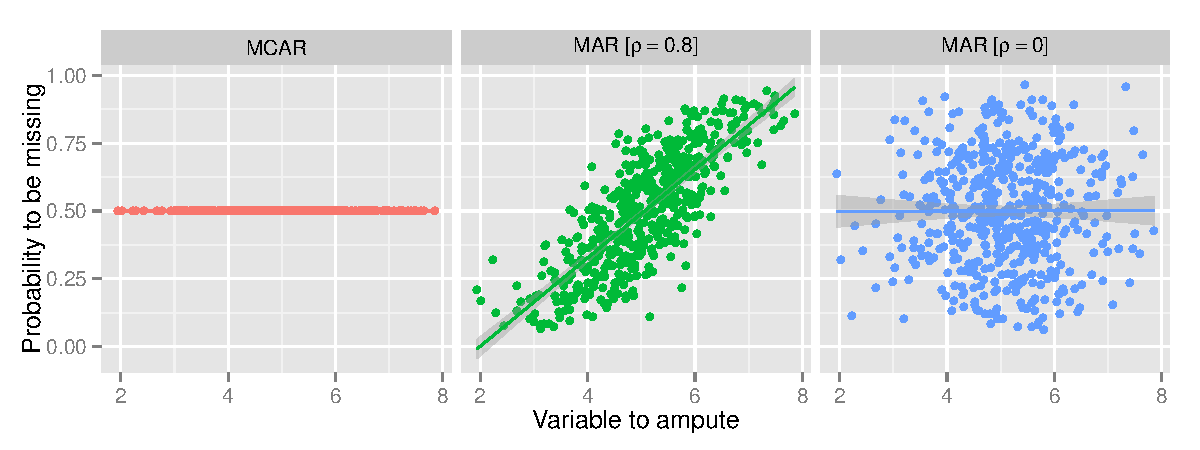
\includegraphics[]{figures/spurious_MAR.pdf}}
\caption{Three missingness mechanisms that yield approximately 50 percent missingness ($N=500$). Displayed are a MCAR mechanism, a right-tailed MAR mechanism generated from bivariate normal data with correlation $\rho=.8$ and the same MAR mechanism, now generated from bivariate normal data with correlation $\rho= 0$.}
\end{center}
\label{fig:MAR}
\end{figure}
\vspace*{1pc}

It is obvious that the MAR missingness generated from data with low correlation would yield similar inference to the MCAR missingness, even though the missingness is random. In fact, this would amount to one of the special cases under which complete case analysis would be more efficient than multiple imputation \citep[see e.g.][p. 48]{fimd}: the missingness does not depend on the incomplete variable. This property might be useful in practice, but considering it as a condition to evaluate performance under MAR missingness is useless. 

Although one cannot definitively verify if the missingness is random - after all, for every MNAR mechanism there is a MAR mechanism with equal fit \citep{molenberghs2008every} - it can be argued that MNAR is the more likely mechanism for real life missingness scenarios. In such cases, an indication of the validity of the obtained inference, given that the assumed missingness mechanism is suspected to be invalid, may be obtained by performing sensitivity analysis \citep[see e.g.][part 5]{molenberghs2014handbook}.

%%%%%%%%%%%%%%%%%%%%%%%%%%

\subsection{Performance evaluation problems}

[Add bridge from last section. And explain how this part is subdivided: first general characteristics of the imputations such as convergence, then performance measures.]

[Performance of different imputation methods may be influenced by preconditions of the methods themselves. All imputation models should be congenial, but this is difficult to test to often ignored even in single imputation endeavor, let alone in simulation studies with 100s of imputations. Same goes for convergence: FCS is iterative and requires algorithmic convergence, but this is typically evaluated through visual inspection which is unfeasible in simulation studies. Ignoring congeniality may yield sub-optimal imputations, which may disadvantage certain methods compared to others.]

Moreover, the performance of imputation procedures on distributional properties is often ignored in simulation studies, and even though the estimates on the analysis level may be justified, some methods can yield imputations that may seem completely invalid to applied researchers. For example, one could very accurately estimate average human height by filling in negative values and values that are unrealistically large. While the obtained inference could still be valid under such imputations, the plausibility of the imputed values given the observed data should be under scrutiny. Rather, one would prefer an imputation technique to yield both valid inference and plausible imputations. It should be studied if an imputation method is prone to deliver such impractical results, and if so, under what conditions.

[Then onto the performance measure part.]

The evaluation criteria used to assess imputation performance vary from one developer to another. This is not surprising as people from different fields could have a different focus on the problem at hand. But the choice of performance measure(s) may inadvertently distort statistical properties of the imputed data.

Developers often only inquire about the 'accuracy' (i.e. how well can the method reproduce the original data). [Add RMSE at cell level here?] The goal of multiple imputation is not to reproduce the data, but to allow for obtaining valid inference given that the data are incomplete. We are interested in the correct answer to the research question; not in the truth itself. This means that, given the framework provided by \citet{rubi87}, statistical properties such as bias, confidence intervals and the coverage rate of the confidence intervals should be studied. After all, the 95\% confidence interval should contain the `true' value at least 95 out of 100 times \citep[][p. 591]{neym34}. [So, what could go wrong by focusing on accuracy exclusively?]

[Add choice of analysis model/estimand here, since performance measure are defined wrt the estimand, e.g., focusing on univariate estimates may favor invalid ad hoc methods.]

[Add problems with RMSE here. And that if the goal is inference (not prediction) then you need appropriate uncertainty, so m = 1 does not suffice.]

Sampling variation has always been an essential part of the evaluation of multiple imputation methodology. However, in order to obtain information about a method's ability to handle the missing data problem, or to objectively compare methods on their ability to correct for missingness, it is not necessary to take sampling variation into account \citep{vink14}. After all, we are interested only in the missing data mechanism, and are not considering the noise induced by the sampling mechanism for evaluation in such studies.

Last, when the evaluator is on the verge of drawing conclusions about the performance of the imputation routine, the performance should be carefully qualified. Comparing the performance of an imputation routine given a population (or true) parameter allows for quantitative evaluation. However, in order to pose qualitative statements about the performance on simulated conditions, comparative methodology is required. For example, when claiming that imputation performance is unacceptable when deviations from normality become rather stringent, such performance is highly dependent on the simulation conditions that are used. For a well-balanced judgement about the severity of the performance drop, comparative simulations with e.g. nonparametric models should be executed. A method may perform badly, but if it still outperforms every other approach, it may yet be of great practical relevance.


%%%%%%%%%%%%%%%%%%%%%%%%%%
%% SOLUTIONS
%%%%%%%%%%%%%%%%%%%%%%%%%%

\section{Suggested course of action}

[In geveral, adhere to ADEMP \citep{morr18}. But there are some differences for the specific case of imputation methodology. All of the parts in ADEMP are used, but a bit scrambled up. Table 1 outlines some of the steps to consider in simulation studies focused on evaluating imputation methodology. The rest of this section is ordered based on these steps.]

\begin{table}[htb]
\begin{center}
\caption{Steps to consider in imputation simulation studies.}
\begin{tabular}{lll}
\hline
Step                  & Aspects under consideration \\
\hline
1. Set scope          & Aim(s), missing data method(s) to evaluate, number of simulation \\
                      & repetitions \\
2. Obtain truth       & Data generating mechanism(s), estimand(s), sampling variance \\
3. Induce missingness & Missingness mechanism(s), missing data pattern(s), missingness \\
                      & proportion(s) \\
4. Apply methods      & Imputation model(s), analysis model(s) \\
% Benchmarking, imputation model parameter, estimand
5. Evaluate methods   & Imputation model fit, performance measures \\
6. Report             & Text, visualization, checklist, simulation script \\
\hline
\end{tabular}
\end{center}
% \footnotesize{Note. Multiple aspects may be varied across simulation conditions (e.g., using a factorial design with several data generating mechanisms and missingness proportions).}
\end{table}


%%%%%%%%%%%%%%%%%%%%%%%%%%

\subsection{Set scope}

Make aim clear. Choose scope (type of DGM, target) and imputation methods to evaluate. Ideally, perform fully factorial design, see \citet{morr18}. Think about tolerable level of uncertainty to pick a number of simulation repetitions. Think about general set-up: are the missing data methods all applied to the same incomplete dataset in each simulation repetition, or is a new incomplete set created per method?  


%%%%%%%%%%%%%%%%%%%%%%%%%%

\subsection{Obtain truth}

% 1a. choose DGM (if model-based: choose n_obs, n_var, relations between var, var types, etc; if design-based: choose n_obs, missing data handling strategy)
% 1b. decide if sampling variance is needed
% 1c. draw complete sample(s)

[Decide which data genetation mechanism to use and obtain true value of the estimand(s).] In model-based simulation data are drawn from a known probability distribution, so the theoretical parameters under which the samples are obtained serve as the comparative truth in the simulations. In design-based simulation, data are sampled from a sufficiently large set, so the parameters of this specific set serve as the comparative truth in the simulations. 

The design-based approach is often used in situations where a probability distribution is not available, or where real-life data structures are of interest. Applications of design-based simulation are often found in official statistics. A benefit of design-based simulation is the ability to use real-life observed data structures.

For evaluations of model-based simulations, it could be convincing to demonstrate a method's applicability to real-world missing data problems. This can, for example, be achieved by obtaining and imputing a fully observed set of variables, wherein the missingness is mimicked from a similar, incomplete set. Alternatively, an incomplete set could be obtained and truth could be established by removing the incomplete cases from the data. However, the real-world missingness would then be omitted.

The simulator must to decide whether there is a need for sampling variance in the simulations scheme. For situations where sampling variance is not of interest, the sampling process can be omitted and a single complete dataset can simply be obtained from the data generating mechanism. The parameters of that single complete set will serve as comparative truth. This process is computationally convenient, because only a single complete datasets has to be considered during all of the simulations. Use alternative pooling rules for finite population inference \citep{raghunathan2003multiple,vink14}. If sampling variance cannot be omitted from the simulation scheme, draw data repeatedly and apply conventional pooling rules \citep[cf.][p. 76-77]{rubi87}.


%%%%%%%%%%%%%%%%%%%%%%%%%%

\subsection{Induce missingness}

% 2a. choose missingness mechanism(s): at least consider MCAR, vary MAR types
% 2b. choose missing data pattern(s): introduce non-monotone multivariate missingness
% 2c. choose missingness proportion(s): at least consider 10, 25 and 50\%

First, one should always consider MCAR missingness, i.e. the scenario where the missing values are missing at random and the observed values are observed at random. Under MCAR, the statistical properties of the observed data given the missing data are known and any imputation routine that cannot at least mimic the performance of the observed data inference, should be deemed inefficient in the scope of the simulation.  

Next, missing data should be induced conform a model that is dependent on the observed data. A straightforward technique for inducing different forms of univariate MAR missingness is described in \citet[][p. 63]{fimd} and a generalization to multivariate MAR missingness can be found in \citet[][Appendix B]{buur06} and \citet[][\S 5.2.3]{brand1999development}. If the missingness is to be induced in longitudinal data, autoregressive MAR models \citep[e.g. cf.][model 2 and model 3]{shara2015randomly} can be useful.

Third, it is advisable to investigate varying shapes of MAR missingness to achieve a more realistic indication of the robustness of the imputation performance across the range of random missingness. Given the simulated data-distributions, one random missingness model may be far more disastrous to the observed information than another model. This may influence the performance of some (but not necessarily all) imputation routines For example, inference from  hot-deck techniques such as predictive mean matching \citep{little1988missing, rubin1986statistical} may be more severely impacted by large amounts of one-tailed missingness than inference from parametric techniques. It would be a shame to overlook such results due to the focus on a single MAR mechanism. 

Fourth, the amount of missingness must be varied. Remember that missingness is only ignorable under MAR when the parameter of the data is distinct and a-priori independent from the parameter of the missing data process. Under MAR missingness we assume that we may use the observed data to make inferences about the joint (observed and unobserved) data. 

The dependency of the procedure on the assumption under which we obtain inference is only influenced by the amount of missingness. If there is no missingness - or if there is no data, for that matter - the inference does not depend on the assumption. Alternatively, the validity of assumptions become increasingly important when the missingness increases. Since we control the MAR mechanism, the assumption under which we may solve the missing data problem should hold and it is only fair to assess performance under stringent missingness conditions. I therefor propose, for all mechanisms, to evaluate at least the following univariate missingness percentages when evaluating imputation routines:

\begin{itemize}
  \item 10\% missingness: Depending on the size of the data, this percentage can be considered as a lower bound of realistic evaluation. Anything less than 10\% may be of little influence on the true data inference. Performance of a missing data method should at least be acceptable for most missing data problems. 
  \item 25\% missingness: This is a fair amount of missingness and will, depending on the observed data information, have a noticeable influence on the completed data inference. When compared to the condition with 10\% missingness, the inference obtained under 25\% missingness should be less certain (i.e. confidence/credibility interval width should increase), but estimates should still be properly covered and the statistical properties of the missing data method should be sound. In practice, at least to my experience in social sciences and official statistics, 25\% univariate missingness can easily be considered as a realistic missingness percentage. 
  \item 50\% missingness: Performance under 50\% percent simulated missingness will most likely be impacted severely. Depending on how the missingness mechanism interacts with the simulated data, some imputation techniques may yield estimates that are under-covered such that the completed data inference should not be deemed valid anymore. If a method yields acceptable inference under 50\% MAR missingness, we can determine that the statistical properties of the imputation methodology are sound. 
\end{itemize}
Although I limit the focus here to ignorable non-response, the above suggested proportions are equally applicable to simulations under non-ignorable non-response.

Fifth, the used missingness mechanism should be detailed, either graphically or written as a function of the data. Often, when inducing missingness, authors remain vague about the actual missingness mechanism under investigation and, even worse, some authors only report something like
\begin{quote}
\emph{We generated missing data following a MAR missingness mechanism.}
\end{quote}
This should be considered unacceptable as claims about the validity of the multiple imputation inference depends heavily on the simulated missingness mechanism. 

%%%%%%%%%%%%%%%%%%%%%%%%%%

\subsection{Apply missing data method(s) and analysis model(s)}

% 3a. Define missing data methods: at least consider complete case analysis as benchmark
% 3b. Choose imputation model parameters: appropriate n_imp and n_it (if applicable), maybe vary predictor matrices?
% 3c. Impute the data
% 3d. Obtain estimates

%%%%%%%%%%%%%%%%%%%%%%%%%%

\subsection{Step 4. Evaluate performance}

% 4a. Evaluate imputations: check failed methods, algorithmic convergence (if applicable)
% 4b. Check imputation model fit: anomalies in distributionsal characteristics, plausibility of imputed values (if requested), PPC
% 4c. Apply performance measures: at least consider bias, coverage, CI length, if applicable also RMSE (at prediction and/or cell level)

It is wise to evaluate the performance of complete case analysis (aka list-wise deletion) in all simulated conditions. We know the theoretical properties of complete case analysis, which makes the technique useful as a point of departure when evaluating multiple imputation performance. 
The evaluation criteria may depend on the estimand. When descriptive statistics are the goal and when statistical inference would not be of interest, bias of the estimates would still apply, but standard errors are generally ignored. Chances are that for those who focus on descriptive statistical applications, multiple imputation would not be the mode of choice. In general, we would say that each multiple imputation routine should be evaluated on at least the following points:
\begin{itemize}
  \item \emph{Bias:} Results should preferable be unbiased. However, the way bias is considered can greatly influence the interpretation of the results. For example, a negligible absolute bias for a parameter for which the true value is zero, would yield infinite bias when relative bias is considered. The way bias is computed should therefore be carefully chosen and described. 
  \item \emph{Interval width:} The way the confidence interval is calculated should be described. Wider intervals are associated with more uncertainty and the more narrow interval that is still properly covered indicates a sharper inference. However, inference from a wider interval that is properly covered is to be considered more valid when compared to a more narrow interval that is not properly covered anymore. 
  \item \emph{Coverage:} Coverage of a 95\% interval should in theory be $\geq 95$, where a coverage of 95\% would be most efficient. Under-coverage (when estimation is too liberal) may be an indication of invalid inference, while over-coverage (when estimation is too conservative) tells us that efficiency could still be gained. 
  \item \emph{RMSE:} [RMSE at cell level and at prediction level (if applicable).]
  \item \emph{Distributional characteristics:} In practice, the distribution of the incomplete data may differ greatly from the observed data. Under anything but the MCAR assumption, this can be expected. When evaluating imputations, the distributional shapes should be checked and diagnostic evaluations should be performed \citep[see][for an detailed overview of diagnostic evaluation for multivariate imputations]{abayomi2008diagnostics}. When anomalies are found, and if the imputation method is valid, there should be an explanation, especially in the controlled environment of a properly executed simulation study. 
  \item \emph{Plausibility of the imputed values:} Plausible imputations - imputations that could be real values if they had been observed - are not a necessary condition for obtaining valid inference. However, in practice, especially when the imputer and the analyst are different persons, plausibility of imputations may be a desired property. When evaluating imputation routines, the evaluator should mention whether the routine is prone to deliver implausible values. 
  \item \emph{Fit of the imputation model:} [PPC, ref Mingyang, \citep{nguy17, zhao22}.]
  \item \emph{Convergence of the algorithm:} Most contemporary imputation techniques rely on iterative algorithms, such as the Gibbs sampler, where some algorithms are critically considered to be possibly incompatible Gibbs samplers \citep[PIGS,][]{li2012imputing}. The convergence of all iterative algorithms should always be considered and if non-convergence is suspected, the inference resulting from the imputations should not be considered.  
  \end{itemize}
For evaluations of model-based simulations, it could be convincing to demonstrate a method's applicability to real-world missing data problems. This can, for example, be achieved by obtaining and imputing a fully observed set of variables, wherein the missingness is mimicked from a similar, incomplete set. Alternatively, an incomplete set could be obtained and truth could be established by removing the incomplete cases from the data. However, the real-world missingness would then be omitted.

%%%%%%%%%%%%%%%%%%%%%%%%%%

\subsection{Step 5. Report}

Be explicit in choices, better even to share the script directly. 

Describe the simulation textually, use pseudo-code, a flowchart, visualize missingness and simulation results.

Fill in the following checklist.

1. set-up

- aim

- number of simulations

2. data generation

- model vs design based

- data types

- sample vs population (vs bootstrapping??)

- number of observations

- number of variables

- coherence between variables


3. missingness generation

- monotone/univariate vs multivariate

- missingness mechanism

- type of M(N)AR

- missingness proportion 

4. missing data methods

- imputation method

- imputation model

- number of imputations

- number of iterations

5. performance evaluation

- analysis model

- estimand

- diagnostic

- ppc


%%%%%%%%%%%%%%%%%%%%%%%%%%
%% DISCUSSION
%%%%%%%%%%%%%%%%%%%%%%%%%%

\section{Discussion}

This document is aimed at establishing a common ground for the evaluation of imputation routines. Such a common ground would be the basis of a standardized evaluation. This allows for fair and efficient comparisons between imputation techniques. Ultimately, it would be desirable to evaluate every imputation routine against the same standardized set in order to quantify the statistical properties across imputation routines. If properly executed, this would allow for careful matching of imputation methodologies to new missing data problems. 


%%%%%%%%%%%%%%%%%%%%%%%%%%
%% APPENDICES
%%%%%%%%%%%%%%%%%%%%%%%%%%

\begin{acknowledgement}
[Maybe add Gelman here?]
\end{acknowledgement}
\vspace*{1pc}

\noindent {\bf{Conflict of Interest}}

\noindent {\it{The authors have declared no conflict of interest. (or please state any conflicts of interest)}}

% \section*{Appendix {\it(please insert here, if applicable)}}
% 
% \subsection*{A.1.\enspace Second level heading}
% 
% Please insert appendices before the references.

%%%%%%%%%%%%%%%%%%%%%%%%%%
%% REFERENCES
%%%%%%%%%%%%%%%%%%%%%%%%%%
\bibliography{bibliography}
\bibliographystyle{apalike}

% \begin{thebibliography}{10}
% \bibitem[Bauer and Bauer(1994)Bauer, P. and Bauer, M.M.]{bib1}Bauer, P. and  Bauer, M. M. (1994). Testing equivalence simultaneously for location and  dispersion of two normally distributed populations.  \textit{Biometrical  Journal} \textbf{36}, 643--660.
% \bibitem[Farrington, C. P. and Andrews, N. (2003)]{bib2}Farrington, C.P. and Andrews, N. (2003). Outbreak detection:
% Application to infectious disease surveillance. In: Monitoring the Health of Populations (eds. R. Brookmeyer and D. F. Stroup), Oxford University Press, Oxford,\break 203--231.
% \bibitem[Rencher(1998)Rencher, A.C.]{bib3}Rencher, A. C. (1998).  \textit{Multivariate Statistical Inference and Applications}. Wiley, New  York. 
% \end{thebibliography}
% \newpage
% \phantom{aaaa}
\end{document}